\documentclass[12pt, a4paper]{article}
\usepackage[T2A]{fontenc}
\usepackage[utf8x]{inputenc}
\usepackage[english, russian]{babel}
\usepackage{amsmath}
\usepackage{xcolor}
\usepackage{accsupp}
\usepackage{listings}
\usepackage[unicode, colorlinks=true, linkcolor=blue]{hyperref}
\usepackage{geometry}
\usepackage{graphicx}

\definecolor{codegreen}{rgb}{0,0.6,0}
\definecolor{codegray}{rgb}{0.5,0.5,0.5}
\definecolor{codepurple}{rgb}{0.58,0,0.82}
\definecolor{backcolour}{rgb}{0.95,0.95,0.92}
\newcommand{\noncopynumber}[1]{%
    \BeginAccSupp{method=escape,ActualText={}}%
    #1%
    \EndAccSupp{}%
}
\lstdefinestyle{mycodestyle}{
    frame=single,
    backgroundcolor=\color{backcolour},
    commentstyle=\color{codegreen},
    keywordstyle=\color{blue},
    numbers=left,
    numberstyle=\color{codegray},
    breaklines=true,
    basicstyle=\ttfamily,
    breakatwhitespace=false,
    captionpos=b,
    keepspaces=true,
    showspaces=false,
    showstringspaces=false,
    showtabs=false,
    columns=fullflexible,
    numberstyle=\noncopynumber,
    language=C++,
    alsolanguage=PHP
}
\lstset{style=mycodestyle}

\geometry{left=10mm}
\geometry{right=10mm}
\geometry{top=10mm}
\geometry{bottom=20mm}

\graphicspath{{img/}}

\title{\textbf{Лабораторная работа}}
\author{Кербер Егор}
\date{\today}

\begin{document}
\maketitle
%\begin{titlepage}
%    \centering
%    \par
%    \vspace{50mm}
%    {\scshape\Large State University\par}
%    \vspace{10mm}
%    {\scshape\Large Final year project\par}
%    \vspace{15mm}
%    {\huge\bfseries Pigeons love doves\par}
%    \vspace{20mm}
%    {\Large\itshape John Birdwatch\par}
%    \vfill
%    supervised by\par
%    Dr. Mark Brown
%    \vfill
%    {\large \today\par}
%    \vspace{20mm}
%\end{titlepage}
%Text starts here

\tableofcontents
\section*{Цели}
\begin{enumerate}
    \item Доказать существование интеграла
    \item Сделать программу, рисующую и вычисляющую интегральные суммы
    \item Расчитать погрешность
\end{enumerate}
% \newpage
\section{Ход работы}
\subsection{Программа}
\href{https://github.com/Zombie1995/MathIntegralLaba}{https://github.com/Zombie1995/MathIntegralLaba}
\begin{center}
    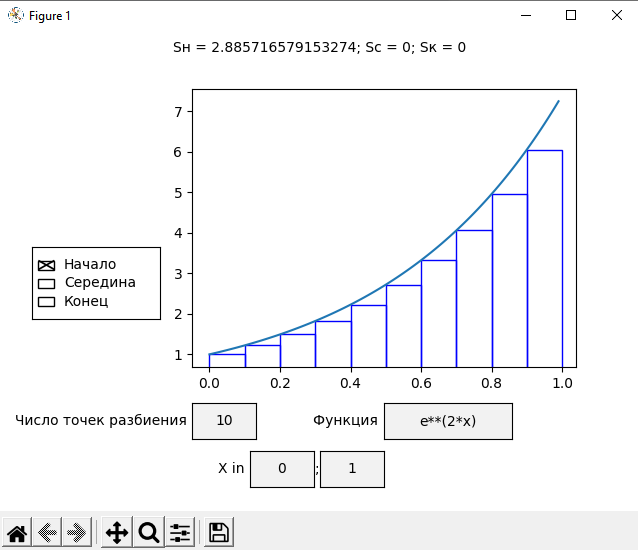
\includegraphics[width=0.35\linewidth]{1}
\end{center}
\begin{center}
    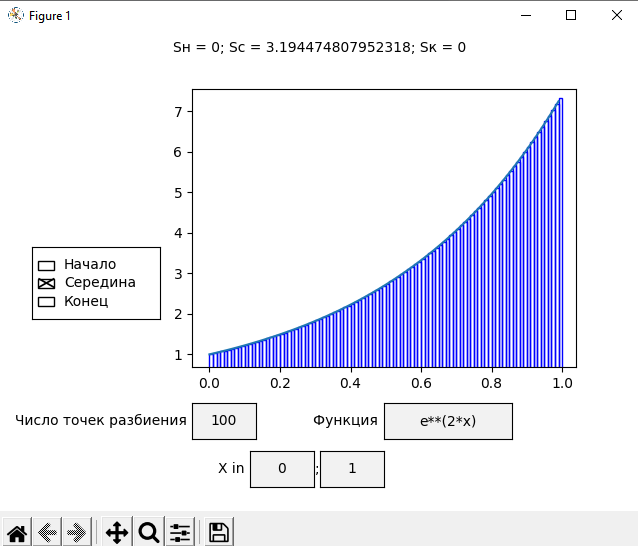
\includegraphics[width=0.35\linewidth]{2}
\end{center}
\begin{center}
    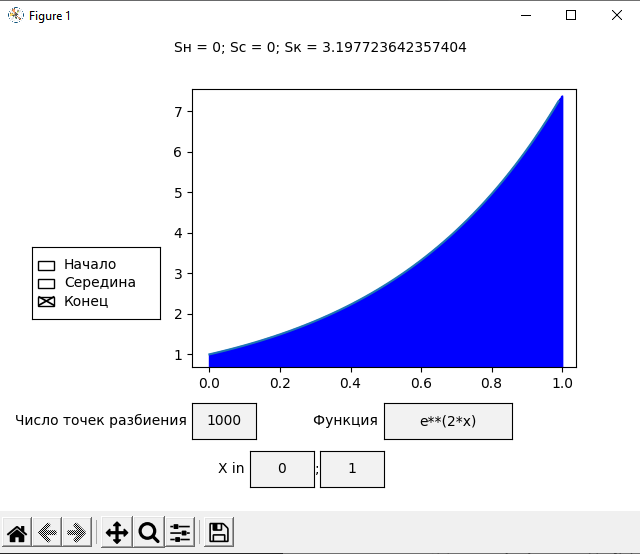
\includegraphics[width=0.35\linewidth]{3}
\end{center}
\begin{center}
    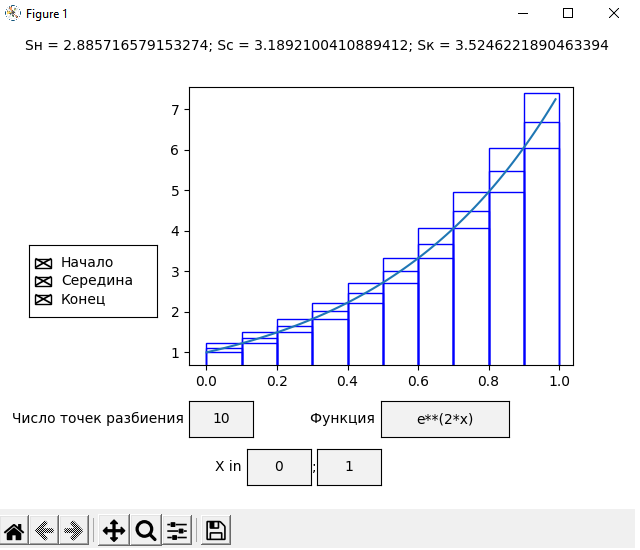
\includegraphics[width=0.35\linewidth]{4}
\end{center}
% \newpage
\subsection{Доказательство существования интеграла}
\begin{equation}
    f=e^{2x}, x\in[0,1]
\end{equation}
\\
\\
\begin{equation}
    \begin{gathered}
        x_k= {k\over n}, k\in N \\
        \overline{S} = \sum\limits_{k=1}^{n} e^{2\frac{k}{n}} \frac{1}{n} = \frac{1}{n} {e^{2\frac{1}{n}} {{1 - e^2} \over {1 - e^{\frac{2}{n}}}}} \underset{n \to \infty}{\longrightarrow} \frac{1}{n} {{1 - e^2} \over -{\frac{2}{n}}} = \frac{e^2}{2} - \frac{1}{2}
    \end{gathered}
\end{equation}
\\
\\
\begin{equation}
    \begin{gathered}
        x_k= {{k - 1}\over n}, k\in N \\
        \underline{S} = \sum\limits_{k=1}^{n} e^{2\frac{k - 1}{n}} \frac{1}{n} = \frac{1}{n} {{1 - e^2} \over {1 - e^{\frac{2}{n}}}} \underset{n \to \infty}{\longrightarrow} \frac{1}{n} {{1 - e^2} \over -{\frac{2}{n}}} = \frac{e^2}{2} - \frac{1}{2}
    \end{gathered}
\end{equation}
\\
\\
\begin{equation}
    |\overline{S}-\underline{S}| \underset{n \to \infty}{\longrightarrow} 0 \implies \exists \int_{0}^{1} f dx
\end{equation}
\\
\\
\begin{equation}
    \int_0^1 e^{2x} dx = \frac{e^{2x}}{2}\bigg|_0^1 = \frac{e^2}{2} - \frac{1}{2}
\end{equation}
% \newpage
\subsection{Погрешность}
\begin{center}
    \(R_n = 2e^{2\xi} (x-x_i)^2\), \\
    \(n = 1\) - степень разложения, \\
    k - число точек разбиения
\end{center}
\begin{equation}
    \begin{gathered}
        \int_0^1 e^{2x} dx = \sum\limits_{i=1}^{k-1}\int_{x_i}^{x_{i+1}} e^{2x} dx = \\
        \sum\limits_{i=1}^{k-1}\int_{x_i}^{x_{i+1}} (e^{2x_i} +2e^{2x_i}(x-x_i) +
        2e^{2\xi} (x-x_i)^2) dx = \\
        \sum\limits_{i=1}^{k-1}\int_{x_i}^{x_{i+1}} e^{2x_i} dx + \sum\limits_{i=1}^{k-1}\int_{x_i}^{x_{i+1}} (2e^{2x_i}(x-x_i) + 2e^{2\xi}(x-x_i)^2)=
        \underline{S} + R \\
        R = I - \underline{S} = \sum\limits_{i=1}^{k-1}\int_{x_i}^{x_{i+1}} (2e^{2x_i}(x-x_i) + 2e^{2\xi}(x-x_i)^2)
    \end{gathered}
\end{equation}
\begin{center}
    Для \(\overline{S}\):
\end{center}
\begin{equation}
    R = \sum\limits_{i=1}^{k-1}\int_{x_i}^{x_{i+1}} (2e^{2x_{i+1}}(x-x_{i+1}) + 2e^{2\xi}(x-x_{i+1})^2)
\end{equation}
Для больших \(n\) можно отбросить \(R_n\) и тогда погрешность будет выражена в более явном виде (возможно).
% \newpage
\section{Вывод}
Интегральные суммы можно использовать для приближенного вычисления интеграла. \\
(Вспомнил Тейлора, хороший был мужик. Интегральные суммы вообще прикольные.)
\end{document}